% The three kinds of transformations in anvl: tracing (R function -> graph), graph -> graph
% (reverse-mode AD), and graph -> executable (the "pjrt" and "quickr" backends). The fill colour
% of a node is the package that implements it. Colours follow the mlr3torch figures.
\documentclass[tikz]{standalone}

\usepackage[utf8]{inputenc}
\usepackage[T1]{fontenc}
\usepackage{lmodern}
\usepackage{tikz}
\usetikzlibrary{positioning, arrows.meta, calc}

\definecolor{tealframe}{HTML}{21908c}
\definecolor{lightbox}{HTML}{e4f1f1}
\definecolor{ltensor}{HTML}{f6f9e4}
\definecolor{viridis1}{HTML}{8e6698}
\definecolor{viridis8}{HTML}{ccea84}
\definecolor{modelgrey}{HTML}{e5e5e5}

\colorlet{cr}{white}
\colorlet{canvl}{lightbox}
\colorlet{cstablehlo}{viridis1!22}
\colorlet{cpjrt}{viridis8!45}
\colorlet{cquickr}{modelgrey}

\tikzset{
  box/.style = {draw = black, rounded corners = 3pt, line width = 0.5pt},
  obj/.style = {box, align = center, font = \footnotesize, minimum height = 1.1cm,
    text width = #1, inner sep = 2pt},
  obj/.default = 2.1cm,
  dev/.style = {box, fill = cpjrt, align = center, font = \footnotesize,
    minimum height = 0.5cm, text width = 1.55cm, inner sep = 1pt},
  flow/.style = {-{Triangle[length = 5pt, width = 5pt]}, black!70, line width = 0.7pt},
  lab/.style = {font = \scriptsize\ttfamily, inner sep = 1pt},
  stage/.style = {font = \footnotesize\bfseries, text = tealframe},
  leg/.style = {box, minimum width = 0.42cm, minimum height = 0.28cm},
}

\begin{document}
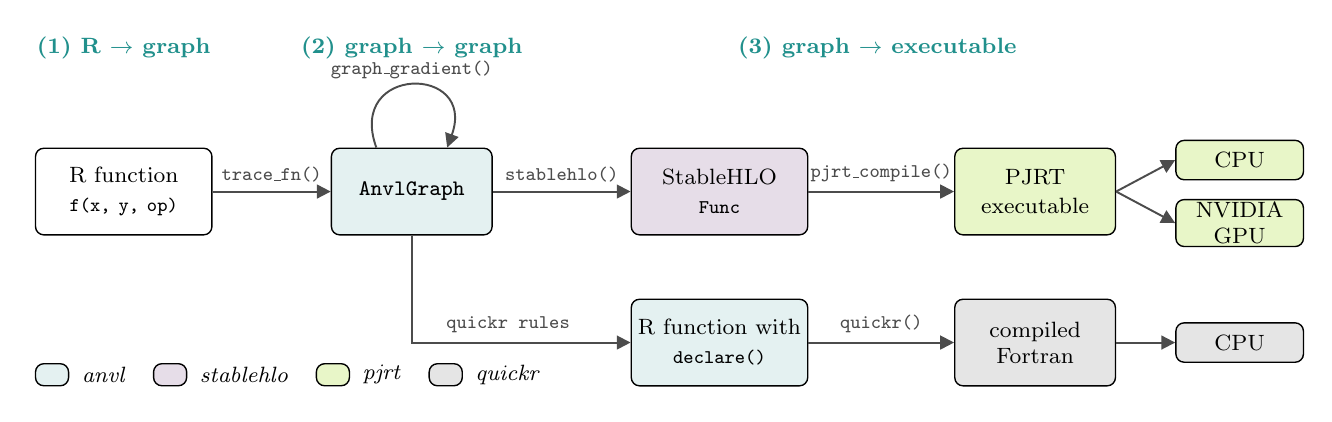
\begin{tikzpicture}

  \node[obj, fill = cr] (fn) {R function\\[1pt]{\scriptsize\ttfamily f(x, y, op)}};
  \node[obj = 1.9cm, fill = canvl, right = 1.5cm of fn] (graph) {\ttfamily AnvlGraph};
  \draw[flow] (fn) -- node[lab, above = 2pt] {trace\_fn()} (graph);
  \draw[flow] ([xshift = -0.45cm] graph.north) to[out = 110, in = 70, looseness = 3.2]
    node[lab, above = 1pt] {graph\_gradient()} ([xshift = 0.45cm] graph.north);

  \node[obj, fill = cstablehlo, right = 1.75cm of graph] (hlo) {StableHLO\\[1pt]{\scriptsize\ttfamily Func}};
  \node[obj = 1.9cm, fill = cpjrt, right = 1.85cm of hlo] (exe) {PJRT\\[1pt]executable};
  \draw[flow] (graph) -- node[lab, above = 2pt] {stablehlo()} (hlo);
  \draw[flow] (hlo) -- node[lab, above = 2pt] {pjrt\_compile()} (exe);
  \node[dev, right = 0.75cm of exe, yshift = 0.4cm] (cpu) {CPU};
  \node[dev, right = 0.75cm of exe, yshift = -0.4cm] (gpu) {NVIDIA GPU};
  \draw[flow] (exe.east) -- (cpu.west);
  \draw[flow] (exe.east) -- (gpu.west);

  \node[obj, fill = canvl, below = 0.8cm of hlo] (qr) {R function with\\[1pt]{\scriptsize\ttfamily declare()}};
  \node[obj = 1.9cm, fill = cquickr, below = 0.8cm of exe] (fortran) {compiled\\Fortran};
  \draw[flow] (graph.south) |- node[lab, above = 2pt, pos = 0.72] {quickr rules} (qr.west);
  \draw[flow] (qr) -- node[lab, above = 2pt] {quickr()} (fortran);
  \node[dev, fill = cquickr, right = 0.75cm of fortran] (cpu2) {CPU};
  \draw[flow] (fortran) -- (cpu2);

  \node[stage, anchor = south] (s2) at ($(graph.north) + (0, 1.0)$) {(2) graph $\rightarrow$ graph};
  \node[stage] at (s2 -| fn) {(1) R $\rightarrow$ graph};
  \node[stage] at ($(s2 -| hlo)!0.5!(s2 -| exe)$) {(3) graph $\rightarrow$ executable};

  \node[leg, fill = canvl, anchor = west] (l1) at ($(fn.west |- fortran.south) + (0, 0.15)$) {};
  \node[font = \footnotesize, right = 1pt of l1] (t1) {\textit{anvl}};
  \node[leg, fill = cstablehlo, right = 6pt of t1] (l2) {};
  \node[font = \footnotesize, right = 1pt of l2] (t2) {\textit{stablehlo}};
  \node[leg, fill = cpjrt, right = 6pt of t2] (l3) {};
  \node[font = \footnotesize, right = 1pt of l3] (t3) {\textit{pjrt}};
  \node[leg, fill = cquickr, right = 6pt of t3] (l4) {};
  \node[font = \footnotesize, right = 1pt of l4] {\textit{quickr}};

\end{tikzpicture}
\end{document}
